
%This section is to clarify the pre-existing tools, defining what was developed in this field until now, and why this tool was used instead of others.

%The general structure is the following:
%\begin{itemize}
%	\item Definition of the specific tool(s) studied (robots, sensor nodes, smart-phones). When relevant, pre-existing experiments.
%	\item Definition of the context of use (indoor/outdoor, humans/animals/robots, with/without connection).
%	\item Definition of used protocols (How the data are collected, when, etc.)
%\end{itemize}

\chapter{Materials and Methods}

This chapter introduced the background and state of the art on multi-robot task scheduling. Chapter \ref{sec:ros_concepts} introduces important concepts of ROS. Chapter \ref{sec:modeling_gazebo} introduces the 3D modeling of robot and environment in Gazebo. Chapter \ref{sec:navigation} introduces robot navigation. Chapter \ref{sec:exist_task_scheduling_methods} introduces previous task scheduling methods. Chapter \ref{sec:cost_function} introduces exist implementation of cost function.

\section{Important Concepts of ROS}
\label{sec:ros_concepts}
ROS is a highly flexible open-source operating system for the robot. It contains various development tools and libraries for developing robot software programs\cite{Pyo17}. It aims to simplify the difficulty and complexity of the process of creating software programs across robot platforms. In this project, ROS is used to archive core autonomous robot functions, including navigation, localization, and mapping.

\subsection{Node}
A ROS node is one executable program. In this project, some existing nodes are used. For instance, the `` move base'' node provides a ROS interface for configuring, running, and interacting with the robot's navigation stack. There are some nodes created for this project, and each node is created for different purposes. For example, one ``Robot controller'' node controls one robot. 

\subsection{Communication Infrastructure}
ROS has a built-in and well-tested messaging system. There are different methods of exchanging messages. ROS topic is a unidirectional anonymous communication. It is used when exchange data continuously. The subscriber receives messages of publisher node only when both of them registered the same topic name. ROS service is bidirectional synchronous communication. The service client requests a service, and the service server responds to the request. The ROS action is a bidirectional asynchronous communication. It is mainly used in two cases. The first case is when it is difficult to use the service due to long response times after the request. The second case is when an intermediate feedback value is needed.
The diagram of message communication is shown in Figure \ref{fig:ros_message_communication}. The messaging system has been applied to this project. For instance, the sensor simulation scenario (Chapter \ref{sec:sensor_simulation}) use ROS Topic method. The communication protocols (Chapter \ref{sec:communication_protocols}) are designed based on the ROS Service method and the ROS Action method. 

\begin{figure}
 \centering
 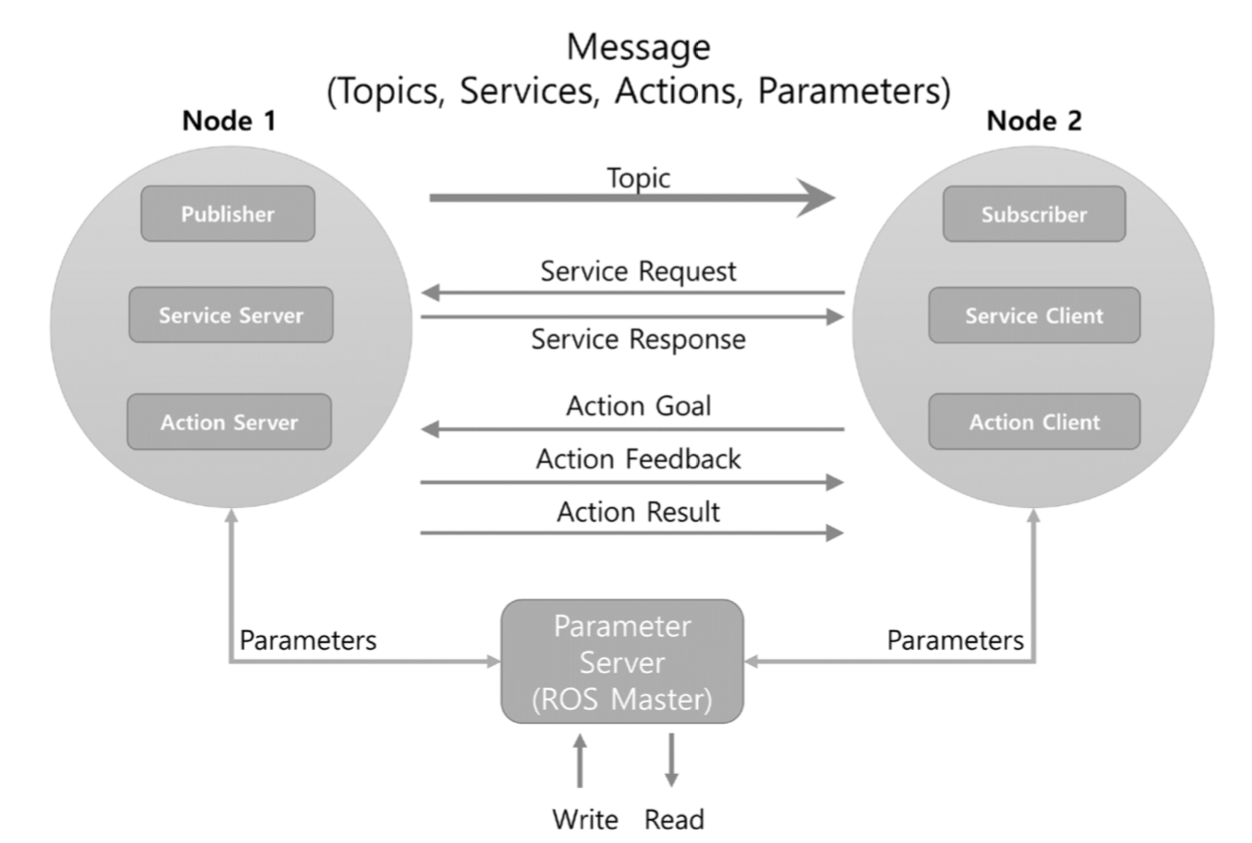
\includegraphics[width = 0.7\textwidth]{content/images/ch2/ros_message_communication.png}
 \caption{ROS Message Communication \cite{Pyo17}}
 \label{fig:ros_message_communication}
 \end{figure}
 
\subsection{ROS Tools}
ROS's core functionality is enhanced by a variety of tools and packages:

\begin{itemize}
 \item \textbf{Rviz.} Rviz\cite{RVIZ} is the 3D visualization tool of ROS. It can visualize information like the distance from a Laser Distance Sensor (LDS) to an obstacle, image value obtained from a camera, Point Cloud Data (PCD) of the 3D distance sensor such as RealSense, Kinect, or Xtion. As is shown in Figure \ref{fig:Rviz_gui}, multiple robot model and its path and laser data can be displayed.
 \begin{figure}[htbp]
 \centering
 \includegraphics[width = 0.7\textwidth]{content/images/ch2/Rviz_gui.png}
 \caption{Rviz Example: Navigation using TurtleBot 3 and Laser Distance Sensor (LDS)}
 \label{fig:Rviz_gui}
 \end{figure}

 \item \textbf{rqt.} rqt is an integration of more than 30 Qt-based ROS GUI development tool. It has plugins such as ``rqt\_tf\_tree'', ``rqt\_plot'' and ``rqt\_graph''
 
 \item \textbf{rqt\_tf\_tree.} rqt\_tf\_tree is a type of rqt. It is a tool for visualizing the tree of topics being broadcast over ROS. Figure \ref{fig:tf_tree} presents the relative coordinate transformation (tf) of multi-robot system. If the poses of Laser Distance Sensor (LDS) are considered as the poses of the robots, the pose information of each robot is connected in the order of odom $\rightarrow$ base\_footprint $\rightarrow$ base\_link $\rightarrow$ base\_scan.
 
 \begin{figure}[htbp]
 \centering
 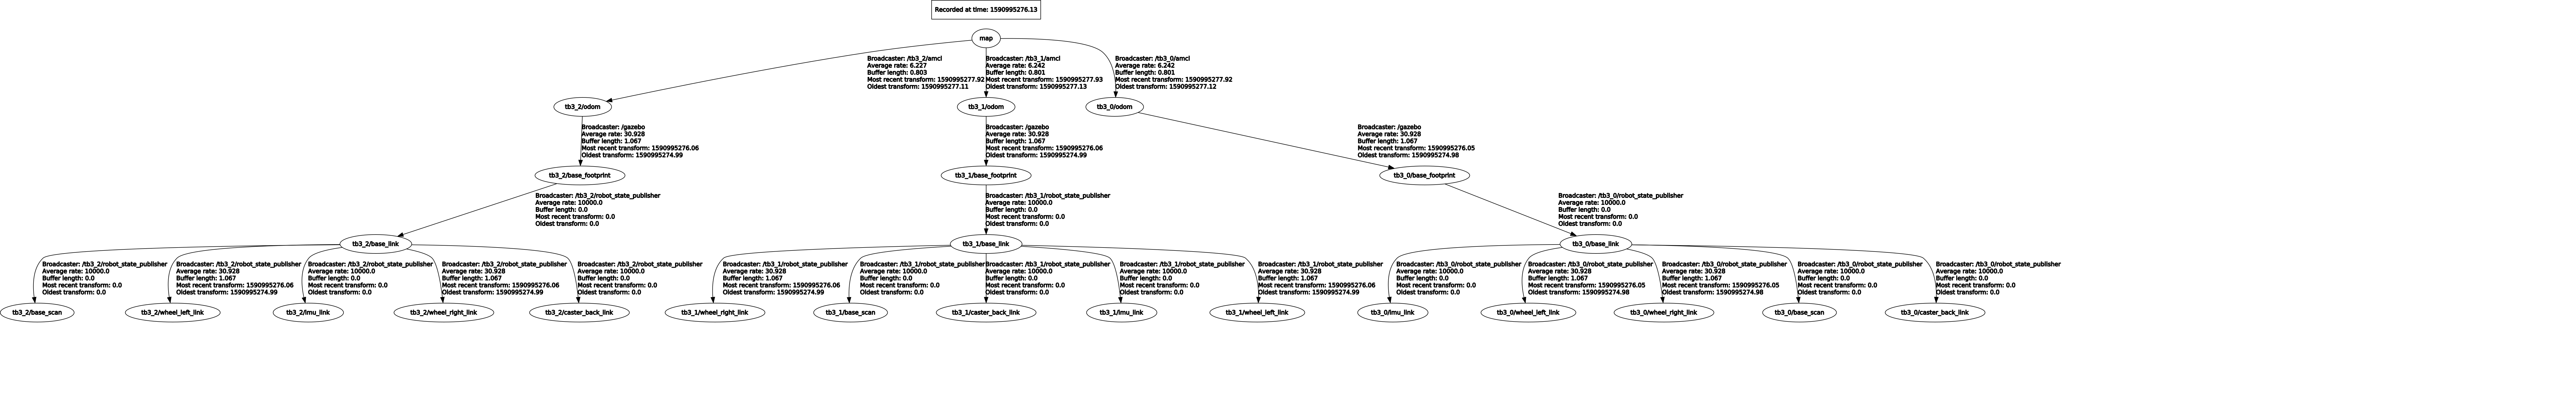
\includegraphics[width = 0.9\textwidth]{content/images/ch2/rqt_tree.png}
 \caption{One Part of rqt\_tf\_tree of the multi-robot system. Each robot has a subtree (like the blue box) and is connected to the map server node }
 \label{fig:tf_tree}
 \end{figure}
 
 \item \textbf{rqt\_graph.} rqt\_graph is a type of rqt. It is a graphical tool that presents the status of nodes and topics. Figure \ref{fig:rqt_graph} presents relation of nodes in multi-robot system.
 \begin{figure}[htbp]
 \centering
 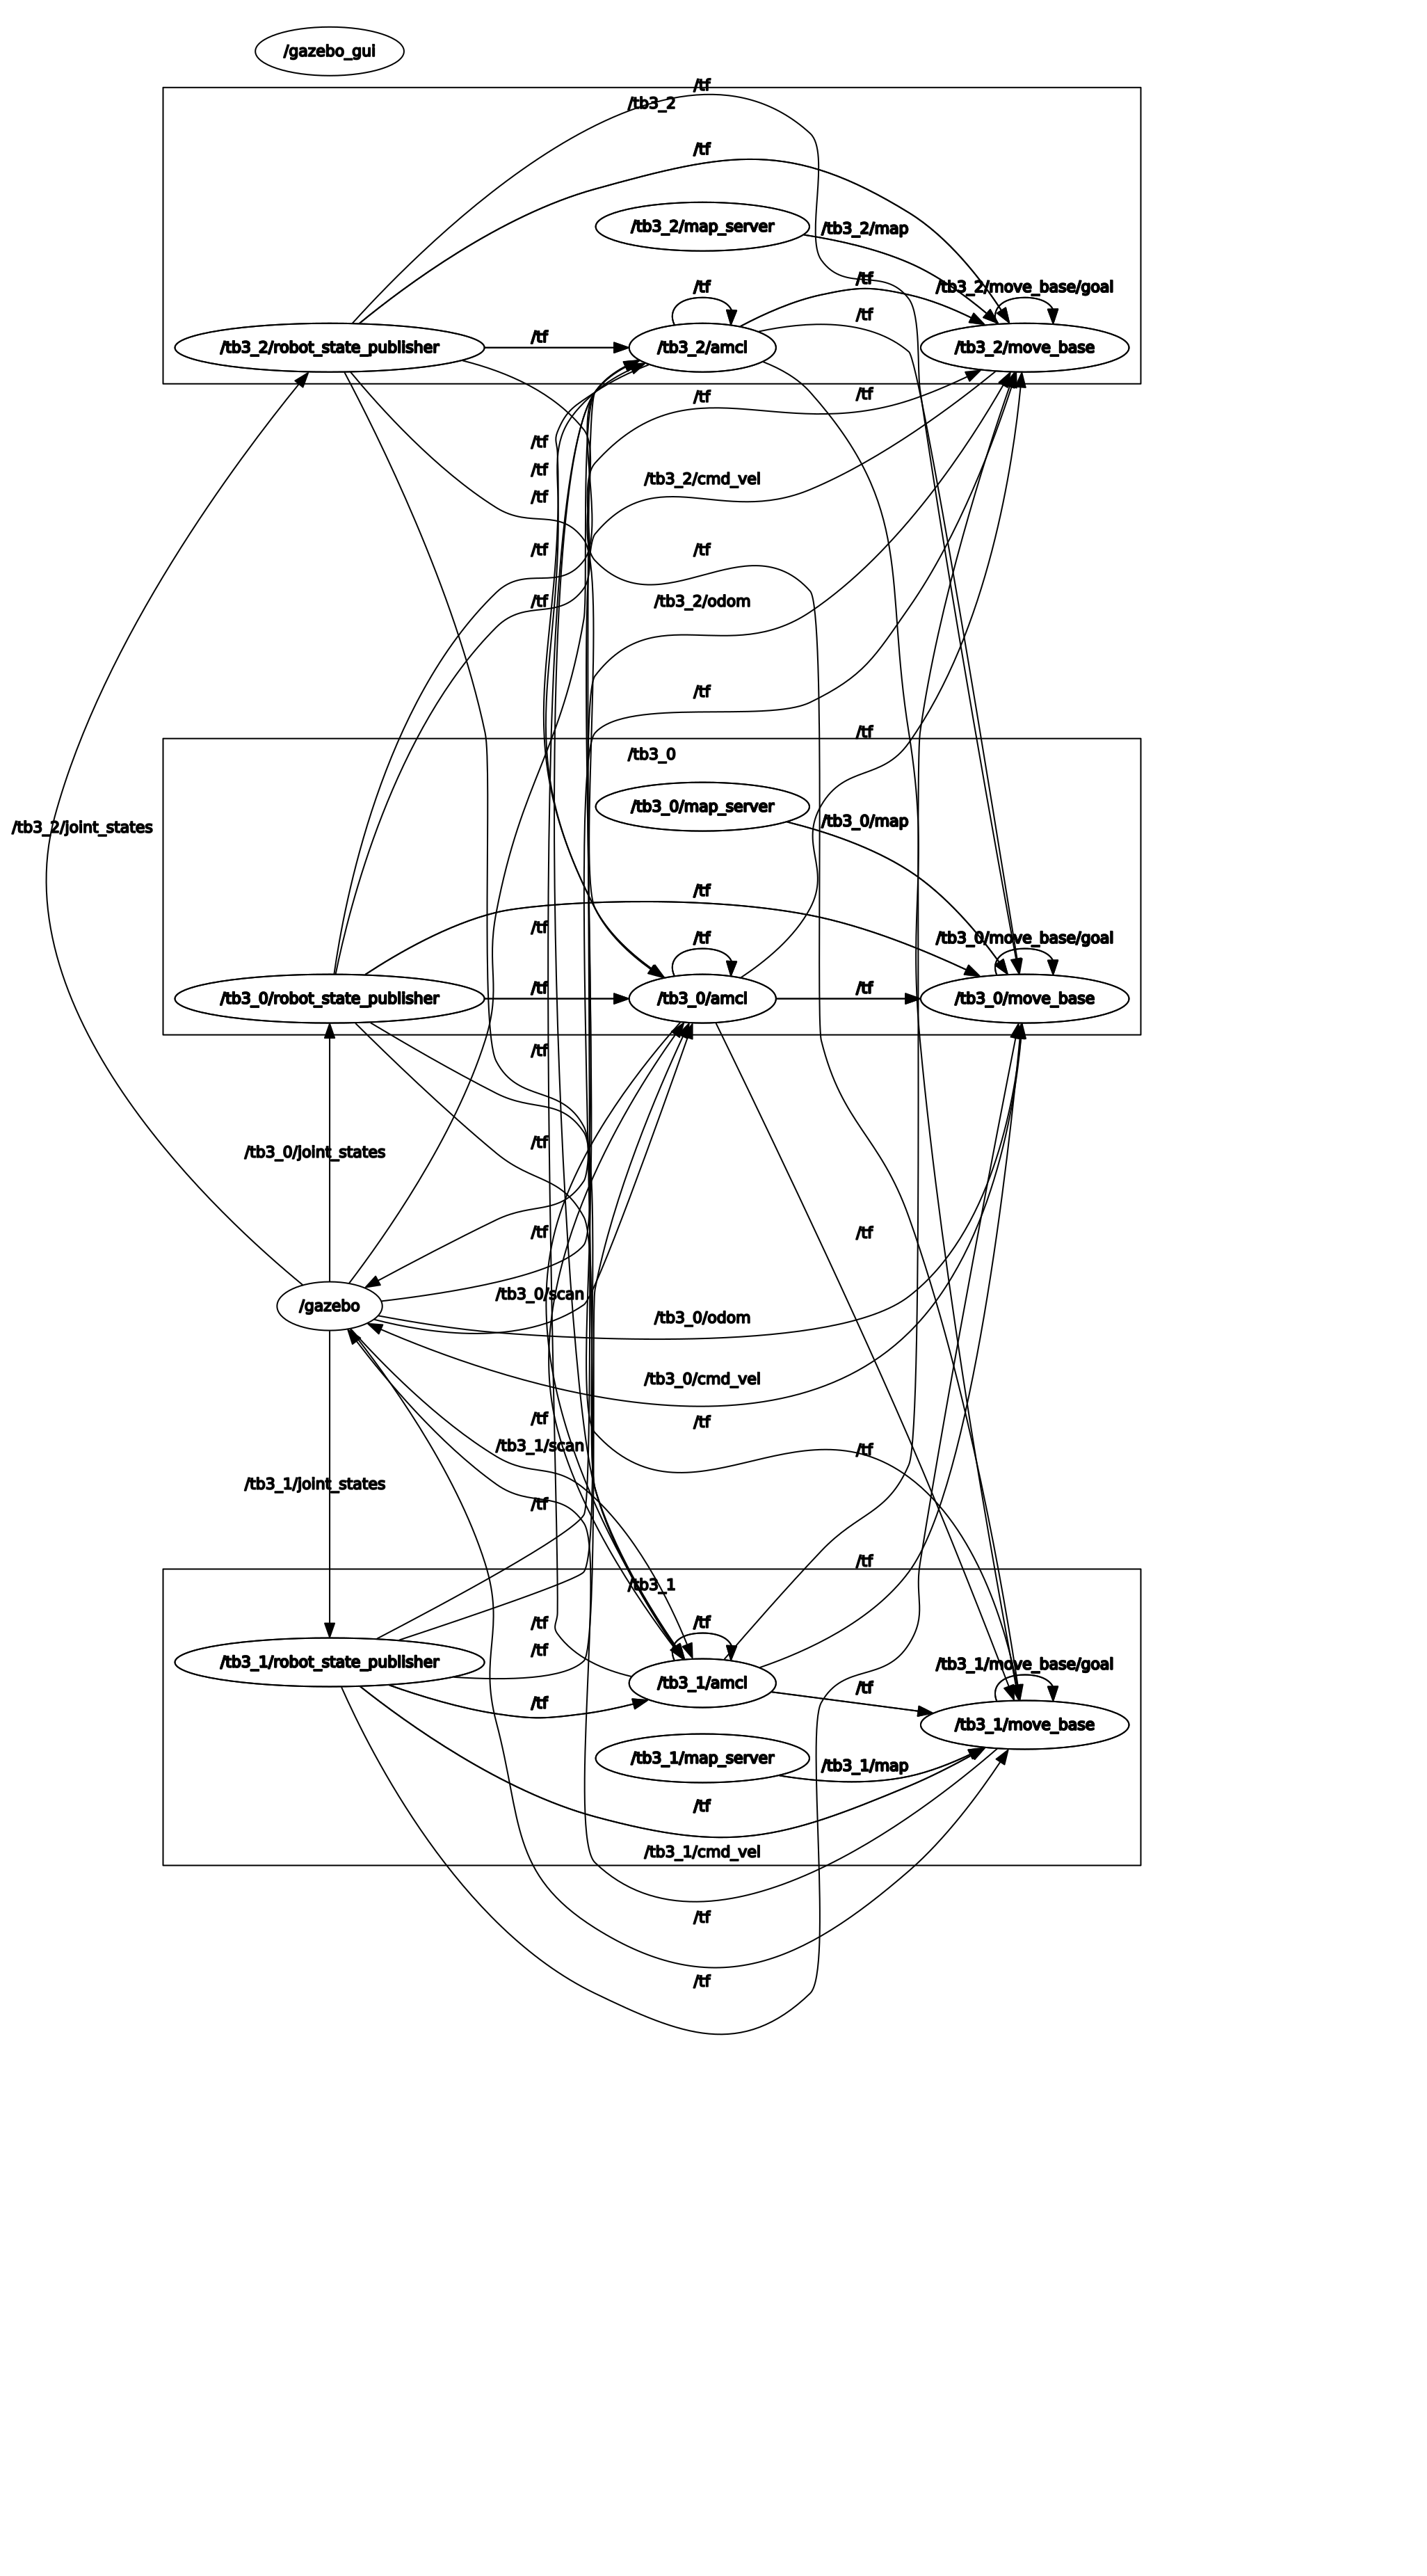
\includegraphics[width = 0.7\textwidth]{content/images/ch2/rosgraph.png}
 \caption{rqt\_graph of multi-robot system}
 \label{fig:rqt_graph}
 \end{figure}

 \item \textbf{Gazebo.} Gazebo \cite{GZ} is the 3D simulation tool integrated with ROS. The details of Gezebo are introduced in Chapter \ref{sec:modeling_gazebo}.
\end{itemize}

\section{TurtleBot3 Simulation Using Gazebo}
\label{sec:modeling_gazebo}

\subsection{Gazebo Simulator}
Robot simulation is essential for robotics research because it can pre-estimate algorithms' performance before applying it to a real robot \cite{Afanasyev2015}. 
The simulator used in this project is Gazebo. Gazebo\cite{GZ} is a 3D robot simulator software based on physics simulation. It is used to simulate the movement of one or multiple robots in complex indoor and outdoor environments.
Using Gazebo, users can create a new 3D model with geometrical primitive or import existing simulated robots and environments. 

\subsection{TurtleBot3 Robot}
The robot model used in this project is TurtleBot3 Burger. TurtleBot3 Burger is a small programmable mobile robot based on ROS. It is widely used in robotics research and education.
As is shown in Figure \ref{fig:robot_hardware}, the basic components are actuators, an SBC (Single-Board Computer) for operating ROS, an LDS sensor for SLAM (Chapter \ref{sec:navigation}) and navigation, restructure mechanism, an OpenCR embedded board used as a sub-controller, sprocket wheels that can be used with tire and caterpillar, and a three-cell lithium-poly battery.
The simulated robot (Figure \ref{fig:simulated_robot}) has a similar outfit. Besides, Gazebo simulates the robot locomotion and sensor measurements used for localization and navigation and exports the simulation results to ROS.


\begin{figure}[htbp]
\centering
\begin{minipage}[t]{0.48\textwidth}
\centering
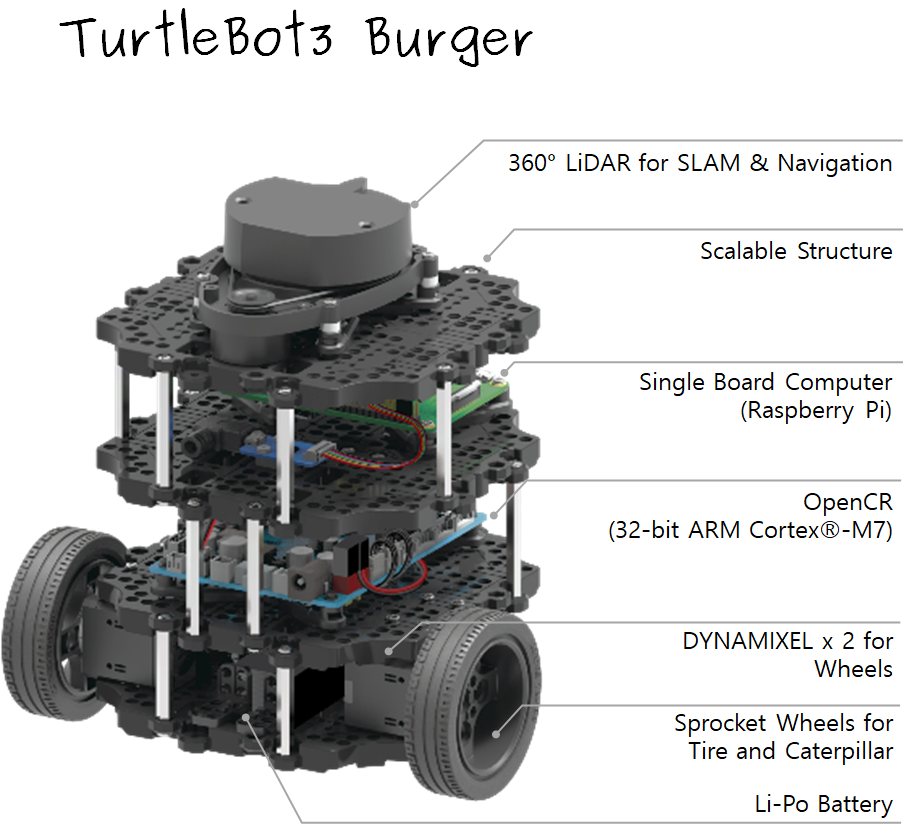
\includegraphics[width=6cm]{content/images/ch2/turtlebot3_burger_components.png}
\caption{Robot Hardware Configuration \cite{Pyo17}}
\label{fig:robot_hardware}
\end{minipage}
\begin{minipage}[t]{0.48\textwidth}
\centering
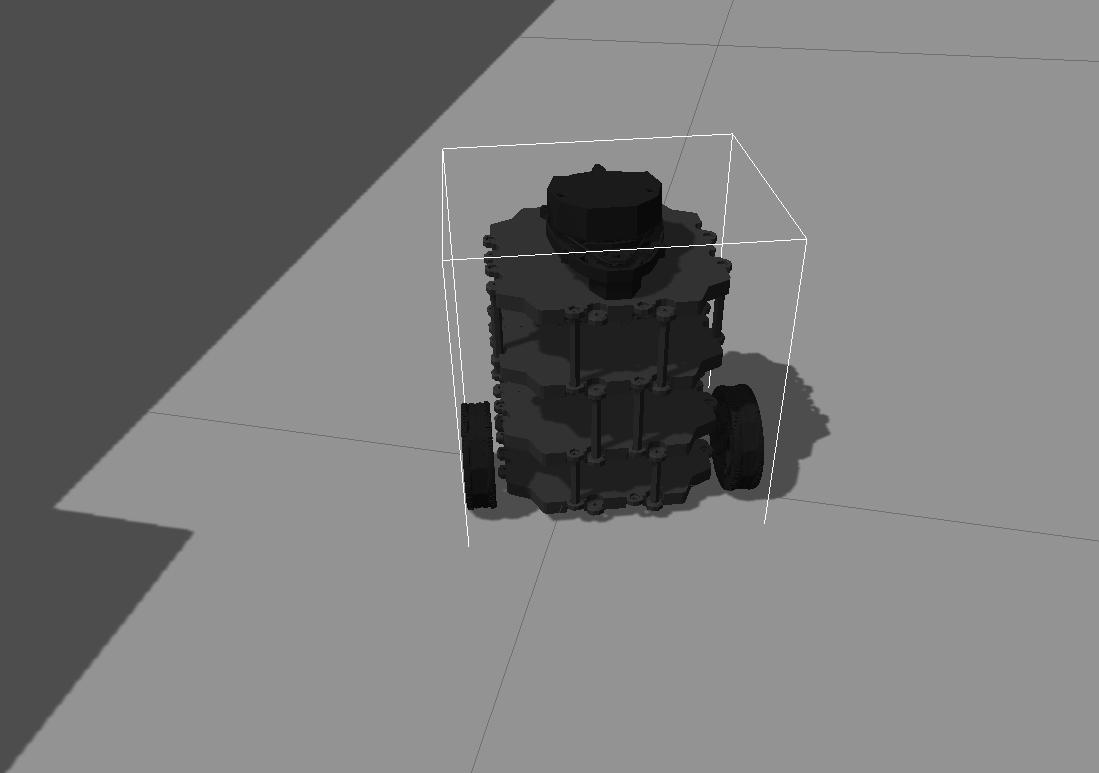
\includegraphics[width=6cm]{content/images/ch2/robot_model.jpg}
\caption{Robot 3D Modeling in Gazebo}
\label{fig:simulated_robot}
\end{minipage}
\end{figure}

\subsection{3D Modeling of the Indoor Environment}

In this project, we selected a model the same as the department's floor as a trial 3D model (Figure \ref{fig:modeling_environment_gazebo}).
This model is a typical office environment that contains a corridor along the central x-axis and 16 rooms located around the corridor. 

\begin{figure}[htbp]
 \centering
 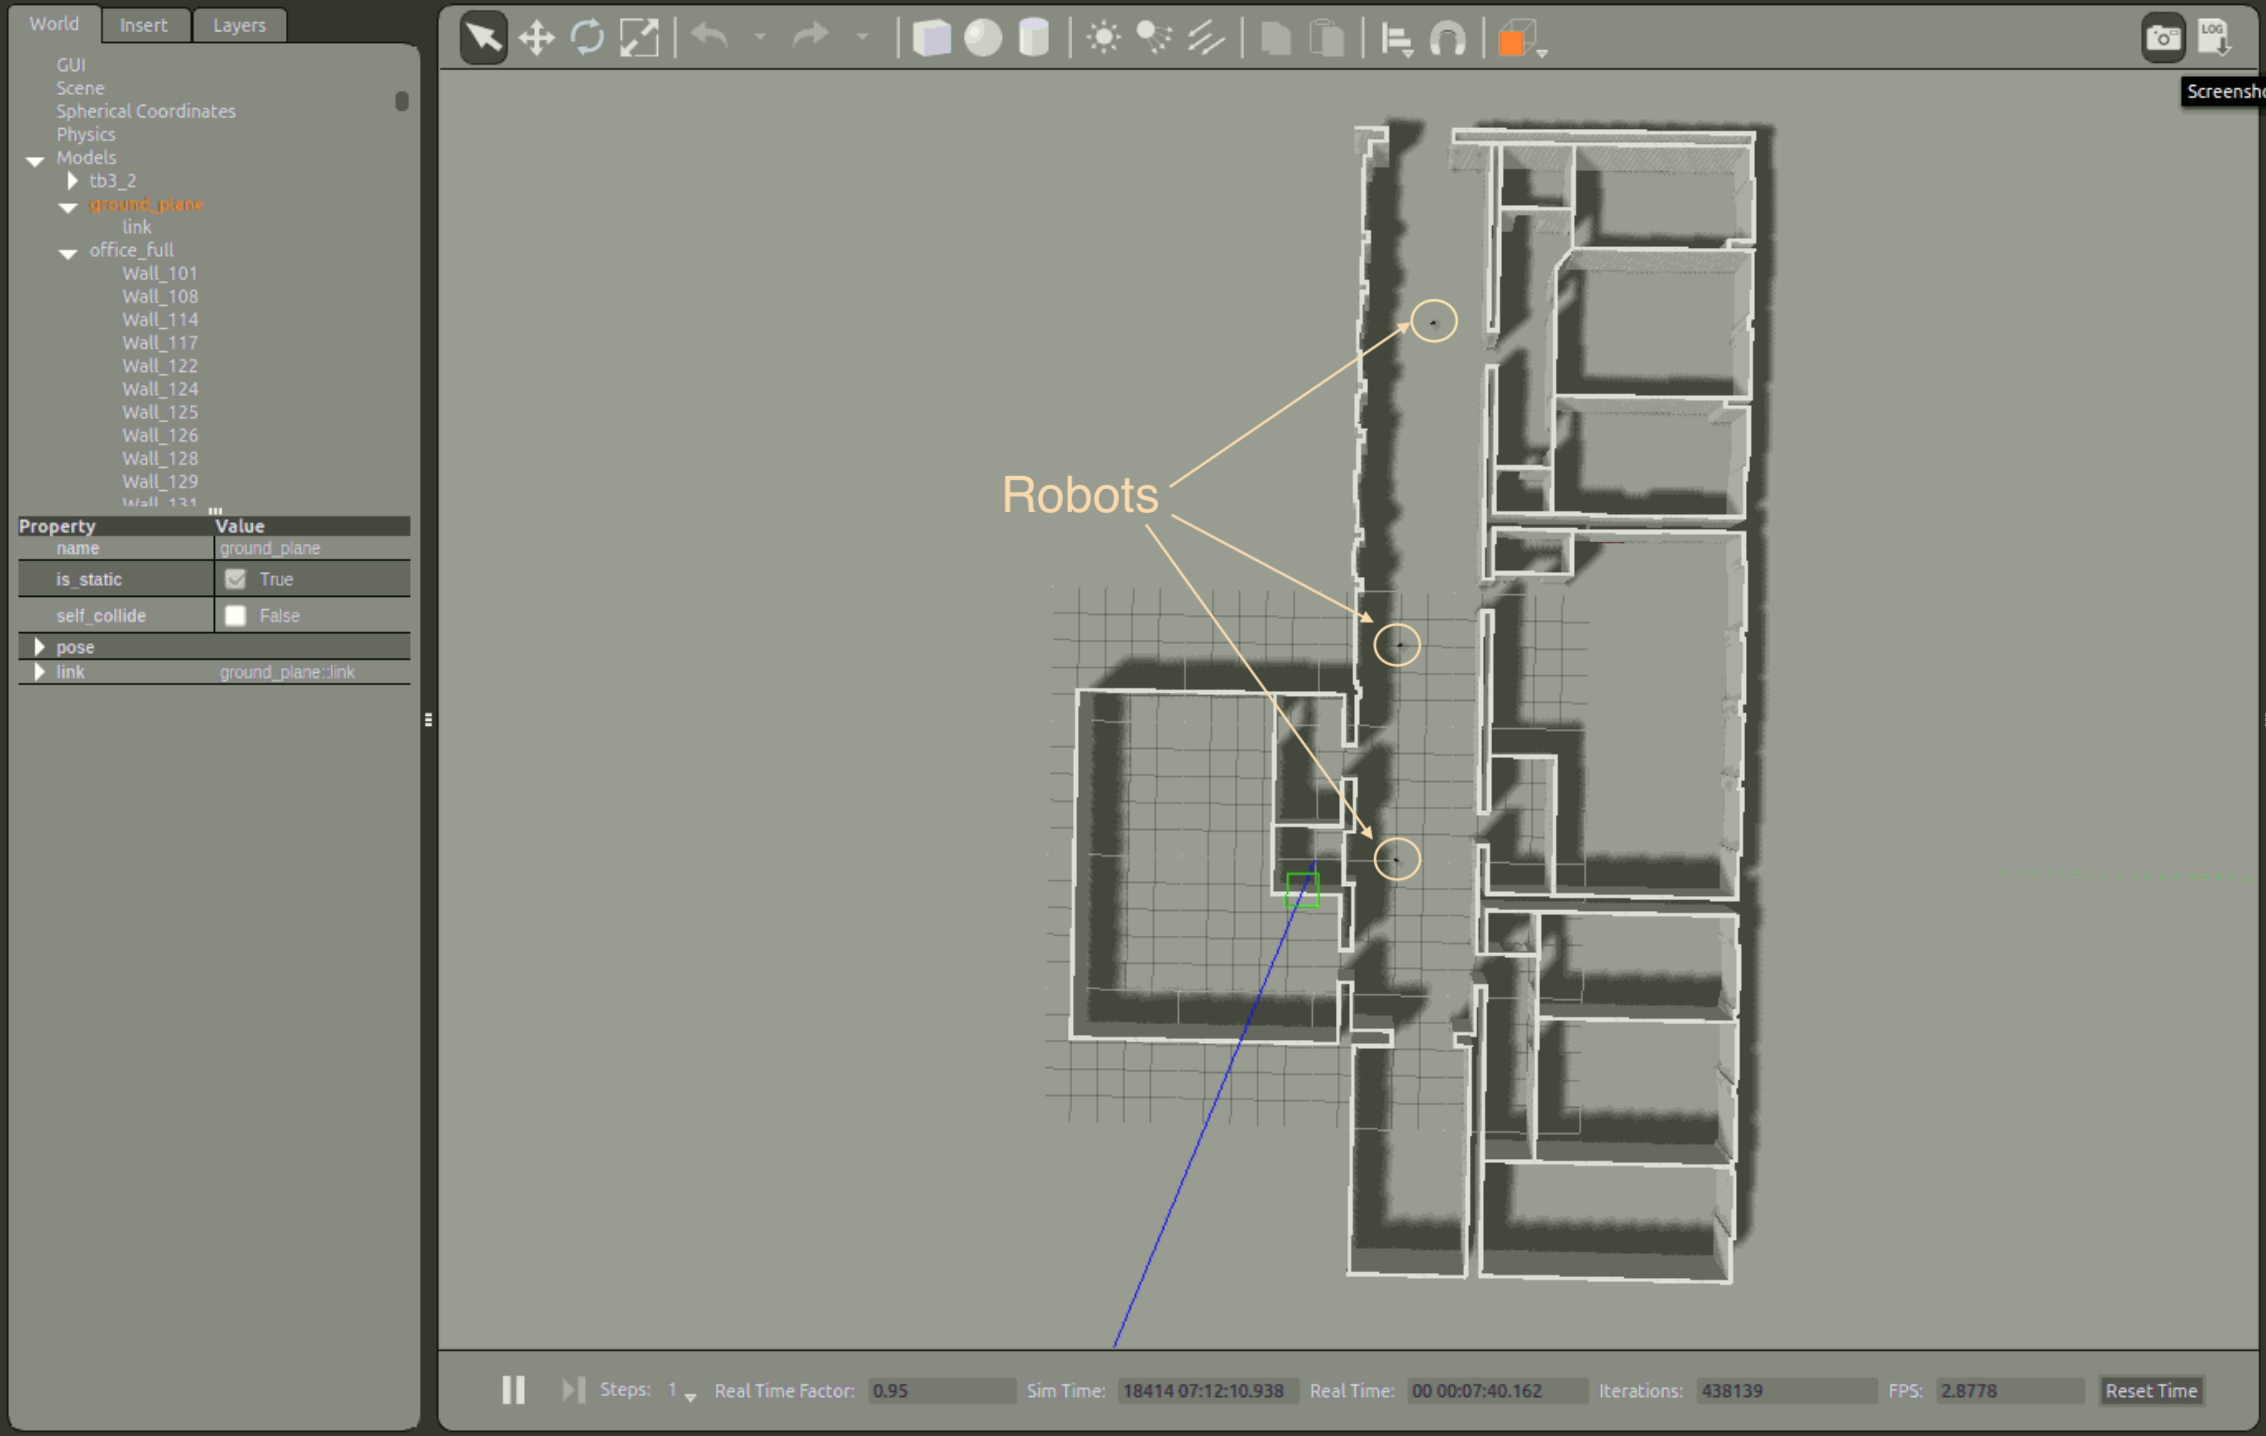
\includegraphics[width = 0.7\textwidth]{content/images/ch2/gazebo_gui_environment.png}
 \caption{3D Modeling of Indoor Environment in Gazebo}
 \label{fig:modeling_environment_gazebo}
\end{figure}

\section{Robot Navigation and Virtual SLAM}
\label{sec:navigation}

There are essential technologies to realize autonomous robot navigation: 
\begin{enumerate}
 \item \textbf{Having a map of the given environment.} In this project, SLAM(Simultaneous Localization And Mapping) is used to create a map of the given environment. Using SLAM, the robot explores the unknown spaces, detects its surrounding areas, estimates its current location, and creates a map. The steps of executing virtual SLAM with TurtleBot3 are shown on the website \cite{T3SLAM}. Once the robot finishes exploring the indoor environment, an occupancy grid map (OCM) is generated (Figure \ref{fig:occupancy_grid}).
 \item \textbf{Measuring or estimating the pose of the robot.} The Pose consists of position and orientation. The dead reckoning \cite{DEADRECKONING} is the most popular indoor pose estimation method for the robot. The amount of movement of the robot is measured with the rotation of the wheel. However, the error between the calculated distance with wheel rotation and the actual travel distance increases over time. Therefore, the inertial measurement unit (IMU) sensor \cite{Woojin17} is used to measure tri-axis angular velocities and tri-axis acceleration to estimate the robot's position. This inertial data can compensate for the error of position and orientation between the calculated value and the actual value.
 \item \textbf{Avoiding obstacles such as walls and furniture.} The laser-based distance sensor on the robot is widely used to determine whether there are obstacles, including walls, furniture, and other robots. The common laser-based distance sensor includes LDS (Laser Distance Sensor), LDF (Laser Doppler Flowmetry), and LiDAR (Light Detection And Ranging) and ultrasonic sensors and infrared distance sensors. The TurtleBot3 equips 360 Laser Distance Sensor LDS-01. The visualization of Laser data in Rviz is shown in Figure \ref{fig:Rviz_gui}.
 \item \textbf{Finding the optimal route calculation and driving.} It is important to find the optimized route to the destination. Many algorithms perform path searching and planning, such as A* algorithm\cite{ASEARCH}, potential field\cite{POTENTIAL}, particle filte\cite{PARTICLE}, and RRT (Rapidly-exploring Random Tree)\cite{RRT}.
 \begin{figure}[htbp]
 \centering
 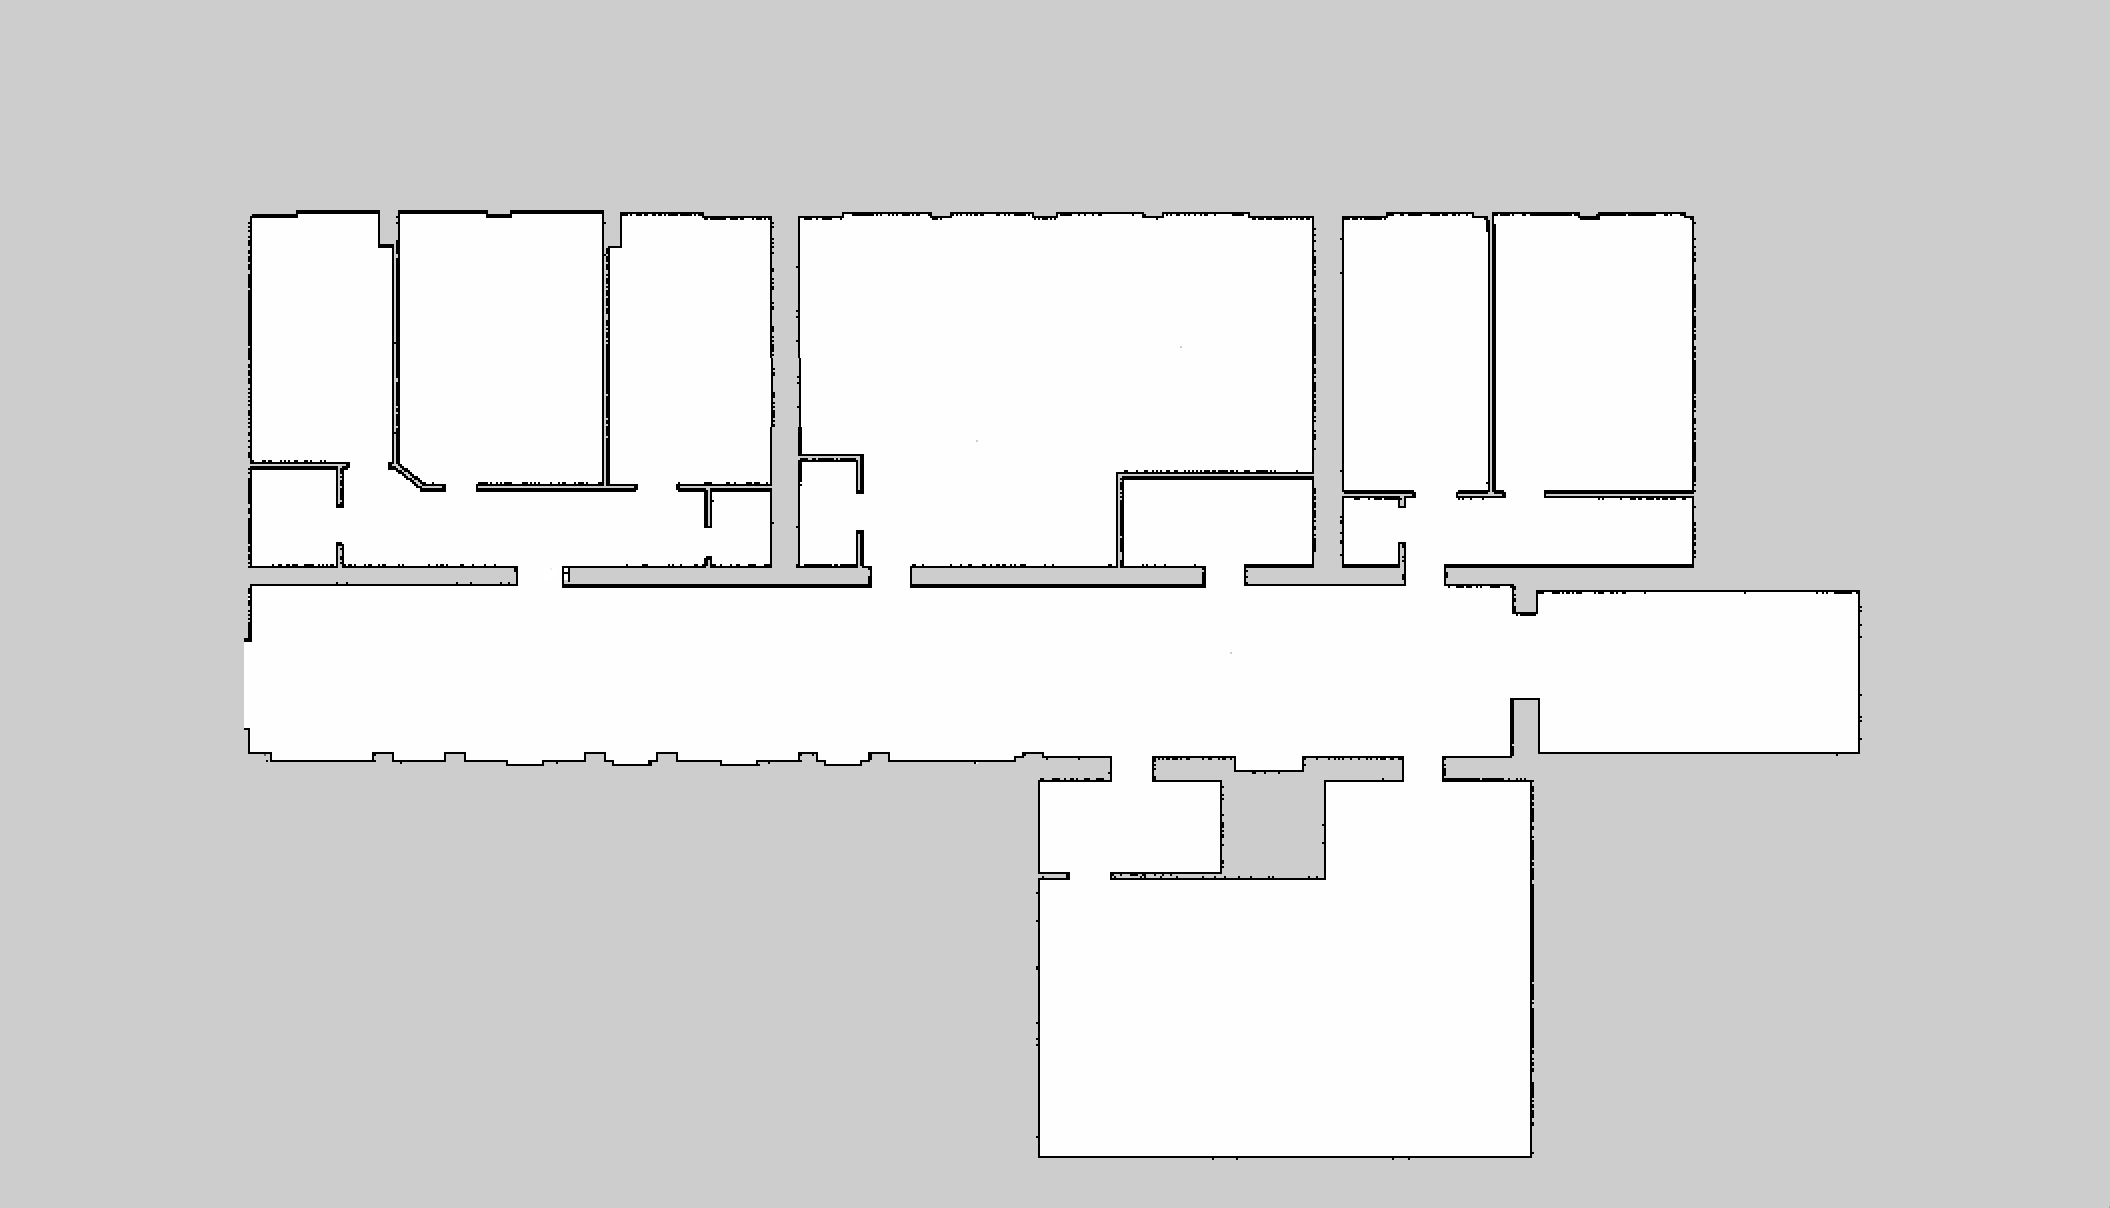
\includegraphics[width = 0.7\textwidth]{content/images/ch2/occupancy_grid.png}
 \caption{Occupancy Grid Map (OGM). White presents the free area in which robots can move, black presents the occupied area in which robots can not move, and gray is the unknown area.}
 \label{fig:occupancy_grid}
 \end{figure}
\end{enumerate}


\section{Task Scheduling Methods}
\label{sec:exist_task_scheduling_methods}
So far, the background information, such as tools and important concepts of ROS, are introduced. This Chapter discusses some popular methods of task scheduling. Those task scheduling methods can be divided into centralized methods and distributed methods.

\subsection{Centralized Method vs. Distributed Method}
In the case of centralized methods, a centralized schedule collects all task requests and uses resource utilization information to schedule tasks. The centralized method is easy to implement and faster to repair in case of failure. However, the robots' autonomy in a pure centralized method is limited because all robots only execute commands from the centralized scheduler and not determine what tasks to do \cite{NUNES201755}. Also, since the centralized scheduler must compute all resources and tasks, the centralized system is difficult to scale to a large-size network \cite{CHRISTODOULOPOULOS20091172}.
Chapter \ref{sec:constraint_programming} introduces a centralized constraint programming method. Chapter \ref{sec:genetic_method} introduces a centralized method based on A* and Genetic Algorithm.

In the case of distributed methods, multiple distributed schedulers keep tracking the resource availability and use this information to perform task scheduling\cite{CHRISTODOULOPOULOS20091172}. This method distributes the associated computation overhead. As a result, it eliminates the bottleneck caused by the centralized scheduler and improves networks' scalability and reliability. The challenge in distributed methods is the coordination of distributed schedulers and the required control plane overhead \cite{CHRISTODOULOPOULOS20091172}.
Chapter \ref{sec:auction_method} introduces a distributed auction method. Chapter \ref{sec:global_unit_method} introduces a communication-efficient distributed method. 

\subsection{Centralized Constraint Programming Method}
\label{sec:constraint_programming}
Booth has proposed a multi-robot system that supports elderly residents in a retirement home setting in \cite{retire2017}. in the morning, the robots search for elderly residents in the retirement home, eliciting their availability and preferences for activities. The centralized scheduler then uses the constraint programming method to allocate these assistive activities over the day. Those problem-specific constraints include robot energy consumption, activity priority, robot-user activity synchronization, user location, and user calendars that identify their available and busy intervals. Once this information is attained, the system allocates and schedules robots for the day before executing the plan.

\subsection{Centralized Method based on A* and Genetic Algorithm}
\label{sec:genetic_method}
Chun has proposed a centralized task scheduling and path-planning method based on A* and Genetic Algorithm \cite{Chun12}.
In this research work, the Genetic Algorithm is responsible for task scheduling to find the optimal solution for industrial plant inspection problems. A* Algorithm is used to calculate the traveling cost and path-planning of a robot moving from one position to another. It can consider more detailed path conditions such as obstacles, furniture, and terrain conditions. The traveling cost is one evaluation parameter of the fitness function in the Genetic Algorithm, but it is referred to as the completion time in this research. To be more precise, it is the period between the first robot starting its tasks and the last robot finishing its tasks.
The goal of the task scheduling method is to find an ordered set of tasks for robots to minimize the completion time while decreasing the total power consumption.
Two Greedy algorithms are proposed for task assignment. The first one is to find one task for each robot that provides for the minimum completion time in each step to minimize the total completion time. The second one is finding only one robot-task pair that takes the minimum time in each step to decrease the total power consumption. 

\subsection{Distributed Auction Method}
\label{sec:auction_method}
When the system performs a long-term task allocation process, the communication link between the customer agent and robots may be disconnected. These problems may cause a conflict or failed assignment. 
Distributed methods are more suitable in this case to distribute the computation to individual agents \cite{NUNES201755}. 
Dong-Hyun Lee has proposed a resource-oriented, distributed auction algorithm \cite{Dong2015}. The customer agents and robots with limited communication ranges construct an ad-hoc network tree. The customer agent becomes auctioneer and broadcasts an auction call to the task. The robots become bidders and submit their bid values to the customer agent. The bid values consider local information such as robot task queue, robot's resource levels, and estimated travel distance and time for multiple paths. Since each path consists of different charging stations, the robot's resource levels after completing a task and estimated travel time depend on the path. After receiving all bid values, the agent assigns the task to the robot with the lowest bid value. This scenarios not only avoids unexpected battery drain while robot processing task, but also let robots maintain high energy.

\subsection{Distributed Method with Global Unit}
\label{sec:global_unit_method}
Kashyap Shah proposed a communication-efficient distributed dynamic task scheduling system with a shared global unit \cite{Shah7}. Each robot can make its own decision by communicating with other robots and checking and updating the current task status in the global unit. Besides, this method considers two unexpected situations. 
Firstly, some robots may be unable to handle their current task because the task environment has changed. In this case, the defective robot checks the global unit and sends a help message to robots that can handle the task. Secondly, some robot may fail in a dynamic environment. This robot failure will be detected by tracking the communication signal, and its status in the global unit will be updated as failed to make sure no more tasks will be allocated to this robot. If the failed robot is running a task, its current task will be reassigned to another robot. 

\section{Cost Function}
\label{sec:cost_function}
One of the most important steps when designing a multi-robot task scheduling algorithm is calculating the tasks' costs. Jia summarizes several physical quantities used in the algorithm's cost in \cite{Jia2013ASA}. In their study, it can be concluded that the most commonly used decision variables are estimated travel distance and time, as proposed in \cite{Dong2015}. Other kinds of decision variables involved are the number of traversals and energy consumed. 
Besides, Korsah proposed a comprehensive taxonomy of multi-robot task scheduling problems that explicitly consider the issues of interrelated utilities and constraints. In this taxonomy, tasks are distinguished by decomposability and multi-agent-allocatability \cite{Korsah13}.
In the case of Chun's method \cite{Chun12}, the cost is defined as completion time. A completion time is calculated for the robot-tasks pairs. The completion time is the time span of the first robot starting its tasks and the last robot finishing its tasks.

